\documentclass{article}
\usepackage{amsmath}
\usepackage{graphicx}
\usepackage{circuitikz}


\title{Hardware Assignment-2}
\author{EE24BTECH11003 - Akshara Sarma Chennubhatla}
\date{March 2025}

\begin{document}
\maketitle
\begin{center}
	\textbf{Assignment:}\\To make a calculator\\with implementation of some\\scientific functions and\\regular BODMAS operations
\end{center}
\vspace{30pt}
\begin{figure}[h!]
	\centering
	
\includegraphics[width = 100pt]{.logo/logo.png}\\
\end{figure}
\begin{center}
	Bachelor of Technology\\
	\vspace{10pt}
	Department of Electrical Engineering\\
\end{center}
\newpage

\maketitle


\tableofcontents
\newpage  

\section{Introduction}
This document details the hardware connections, working principles, and implementation of an Arduino-based calculator. The calculator supports arithmetic operations, scientific functions, and features a scrolling mechanism for selecting trigonometric and logarithmic functions.

\section{Hardware Connections}
\subsection{Microcontroller}
- Arduino Uno

\subsection{Display}
A 16x2 LCD is used for displaying input and results. The connections are as follows:
\begin{itemize}
    \item RS: Pin 2
    \item Enable: Pin 3
    \item D4, D5, D6, D7: Pins 4, 5, 6, 7
\end{itemize}

\subsection{10 -$>$ 1 : Resistor Ladder}
The calculator uses a resistor ladder to read multiple button inputs for digits from 0-9 using a \textbf{SINGLE} analog pin. The principle behind this approach is as follows:
\begin{itemize}
    \item Each button is connected in series with resistors, forming a voltage divider.
    \item When a button is pressed, it changes the resistance in the circuit, altering the voltage read by the analog pin.
    \item The Arduino reads this analog value and maps it to a specific button.
\end{itemize}
This method reduces the number of pins required compared to connecting each button to a separate digital pin.
The circuit of the implementation is as follows:\\
\begin{figure}[!ht]
\centering
\resizebox{1.2\textwidth}{!}{%
\begin{circuitikz}
\tikzstyle{every node}=[font=\normalsize]
\draw (5,15.5) to[R] (6.75,15.5);
\draw (6.75,15.5) to[R] (8.25,15.5);
\draw (8.25,15.5) to[R] (9.5,15.5);
\draw (9.5,15.5) to[R] (11,15.5);
\draw (11,15.5) to[R] (12.5,15.5);
\draw (12.5,15.5) to[R] (13.75,15.5);
\draw (13.75,15.5) to[R] (15,15.5);
\draw (15,15.5) to[R] (16.25,15.5);
\draw (16.25,15.5) to[R] (17.75,15.5);
\draw (17.75,15.5) to[R] (19.25,15.5);
\node at (6.75,15.5) [circ] {};
\node at (8.25,15.5) [circ] {};
\node at (9.5,15.5) [circ] {};
\node at (11,15.5) [circ] {};
\node at (12.5,15.5) [circ] {};
\node at (13.75,15.5) [circ] {};
\node at (15,15.5) [circ] {};
\node at (16.25,15.5) [circ] {};
\node at (17.75,15.5) [circ] {};
\node at (19.25,15.5) [circ] {};
\draw (6.75,15.5) to[push button] (6.75,13.5);
\draw (8.25,15.5) to[push button] (8.25,13.5);
\draw (9.5,15.5) to[push button] (9.5,13.5);
\draw (11,15.5) to[push button] (11,13.5);
\draw (12.5,15.5) to[push button] (12.5,13.5);
\draw (13.75,15.5) to[push button] (13.75,13.5);
\draw (15,15.5) to[push button] (15,13.5);
\draw (16.25,15.5) to[push button] (16.25,13.5);
\draw (17.75,15.5) to[push button] (17.75,13.5);
\draw (19.25,15.5) to[push button] (19.25,13.5);
\node [font=\normalsize] at (3.25,15.5) {$A0 (Arduino)$};
\draw (19.25,13.5) to (20.5,13.5) node[ground]{};
\node [font=\normalsize] at (6.75,15.75) {$0$};
\node [font=\normalsize] at (8.25,15.75) {$1$};
\node [font=\normalsize] at (9.5,15.75) {$2$};
\node [font=\normalsize] at (11,15.75) {$3$};
\node [font=\normalsize] at (12.5,15.75) {$4$};
\node [font=\normalsize] at (13.75,15.75) {$5$};
\node [font=\normalsize] at (15,15.75) {$6$};
\node [font=\normalsize] at (16.25,15.75) {$7$};
\node [font=\normalsize] at (17.75,15.75) {$8$};
\node [font=\normalsize] at (19.25,15.75) {$9$};
\draw (6.75,13.5) to[short] (19.25,13.5);
\draw (5,15.5) to[short] (4.25,15.5);
\node at (4.25,15.5) [circ] {};
\end{circuitikz}
}%
\label{fig:my_label}
\end{figure}

\subsection{Power Supply}
The Arduino can be powered via USB or an external 5V power supply.

\section{Circuit Image}
\begin{figure}[h!]
	\centering
	\rotatebox[origin=c]{90}{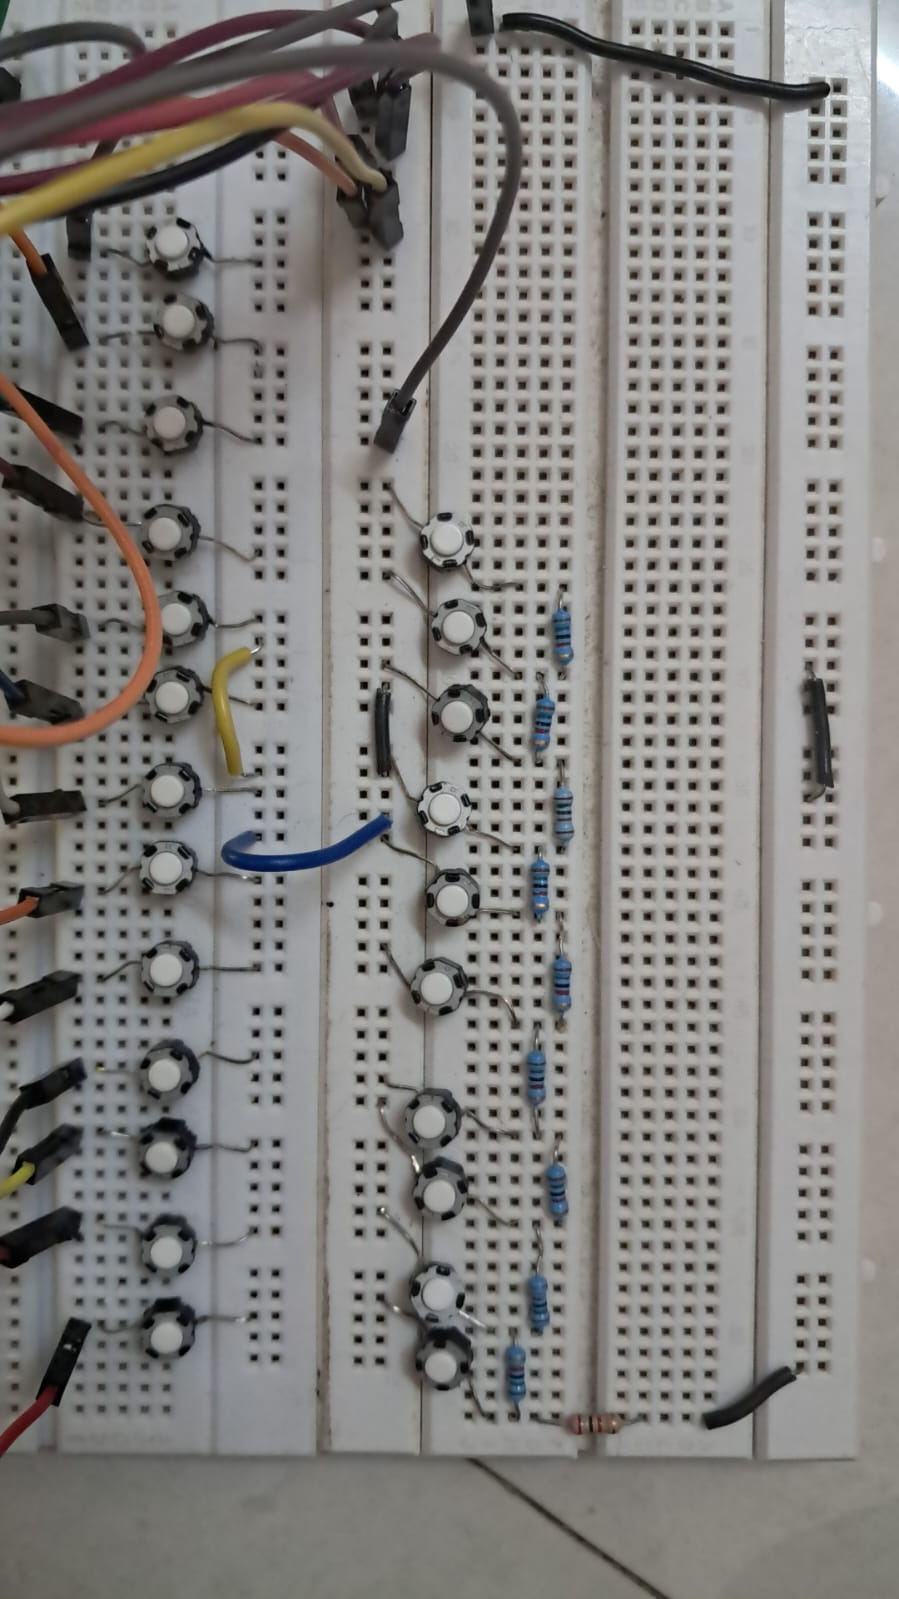
\includegraphics[width = 0.3\textwidth]{figs/circuit.jpeg}}
	\caption{Result-2}
\end{figure}

\section{Working of the Calculator}
\begin{itemize}
\item Uses push buttons as input.
\item LCD displays numbers and operations.
\item Supports basic arithmetic ($+, -, \times, \div$) and scientific functions ($\sin, \cos, \tan, \ln, \log_{10}, pow()$).
\item Includes a temporary answer storage.
\item Implements operator precedence using stacks.
\end{itemize}

\section{Functions and Implementation}
\subsection{Stack Operations}
Stacks are used for handling operator precedence and evaluating expressions.
\begin{itemize}
    \item `initStack()`, `initNumStack()`, `push()`, `pop()`, `peek()`, `isEmpty()` for operator stack.
    \item `pushNum()`, `popNum()` for numerical evaluations.
\end{itemize}

\subsection{Expression Evaluation}
\begin{itemize}
	\item Converts infix expressions to postfix using the \textbf{Shunting Yard Algorithm}.
	\item Evaluates postfix expressions using a number stack.
	\item Handles exponentiation using `pow()`.
	\item Implements a parsing function to read input expressions character by character.
	\item Detects operator precedence dynamically.
	\item Uses a loop to traverse the expression and determine operand boundaries.
\end{itemize}

\subsection{Trigonometric functions Using RK4}
- Trigonometric functions ($\sin, \cos, \tan$) are implemented using the Runge-Kutta 4th Order Method (RK4).

\subsubsection{Runge-Kutta 4th Order Method for $\sin(x)$ Using a Second-Order Differential Equation}
The function $\sin(x)$ satisfies the second-order differential equation:

\begin{equation}
    \frac{d^2 y}{dx^2} + y = 0.
\end{equation}

To solve this using the Runge-Kutta 4th Order Method (RK4), we rewrite it as a system of first-order equations. Let:

\begin{align}
    y_1 &= y = \sin(x), \\
    y_2 &= \frac{dy_1}{dx} = \cos(x).
\end{align}

Thus, the system becomes:

\begin{align}
    \frac{dy_1}{dx} &= y_2, \\
    \frac{dy_2}{dx} &= -y_1.
\end{align}

Applying RK4, we calculate four intermediate values for each step:

\begin{align}
    k_1^1 &= h y_2, \\
    k_1^2 &= h (-y_1), \\
    k_2^1 &= h \left(y_2 + \frac{k_1^2}{2} \right), \\
    k_2^2 &= h \left(-\left(y_1 + \frac{k_1^1}{2} \right) \right), \\
    k_3^1 &= h \left(y_2 + \frac{k_2^2}{2} \right), \\
    k_3^2 &= h \left(-\left(y_1 + \frac{k_2^1}{2} \right) \right), \\
    k_4^1 &= h \left(y_2 + k_3^2 \right), \\
    k_4^2 &= h \left(-\left(y_1 + k_3^1 \right) \right).
\end{align}

The updated values for the next step are:

\begin{align}
    y_1^{n+1} &= y_1^n + \frac{1}{6} (k_1^1 + 2k_2^1 + 2k_3^1 + k_4^1), \\
    y_2^{n+1} &= y_2^n + \frac{1}{6} (k_1^2 + 2k_2^2 + 2k_3^2 + k_4^2).
\end{align}

Since $y_1 = \sin(x)$ and $y_2 = \cos(x)$, this method numerically solves $\sin(x)$ with high accuracy.\\

To calculate $\cos(x)$ we calculate $\sin(\frac{\pi}{2} - x)$\\
To calculate $\tan(x)$ we calculate $\frac{\sin(x)}{\sin(\frac{\pi}{2} - x)}$\\


\subsection{Logarithmic Functions}

\begin{itemize}
	\item The differential equation used is:
\begin{align}
    \frac{d}{dx} \ln(x) &= \frac{1}{x}.
\end{align}
 and the similar RK4 method is applied for finding the value of $\ln(x)$
\item To calculate $\log_{10}(x)$ we use $\frac{\ln(x)}{\ln(10)}$
\end{itemize}


\subsection{Power Function Implementation via Integration}
The function $x^n$ is implemented using the differential equation:

\begin{equation}
    \frac{dy}{dx} = n y
\end{equation}

which follows from the definition of exponentiation. 

\subsubsection{Derivation}
Rearranging the equation:

\begin{equation}
    \frac{dy}{y} = n \, dx
\end{equation}

Integrating both sides from $x = 0$ to $\ln x$:

\begin{equation}
    \int \frac{dy}{y} = \int n \, dx
\end{equation}

\begin{equation}
    \ln y = n x + C
\end{equation}

Setting the initial condition at $x = \ln x$ (since we are computing $x^n$),

\begin{equation}
    \ln y = n \ln x
\end{equation}

Exponentiating both sides:

\begin{equation}
    y = e^{n \ln x}
\end{equation}

which simplifies to:

\begin{equation}
    x^n = e^{n \ln x}
\end{equation}

\subsubsection{Implementation in Code}
The function is computed using the natural logarithm and exponentiation:

\begin{verbatim}
double power(double x, double n) {
    if (x <= 0) return -1;  // Only valid for positive x

    double y = 1.0;  // Initial condition: y(0) = 1
    double log_x = log(x);  // Compute ln(x)
    int steps = abs(log_x / STEP_SIZE);  // Compute number of steps dynamically

    double dx = log_x / steps;  // Adjust step size to match ln(x)


    for (int i = 0; i < steps; i++) {
        y += dx * (n * y);  // Euler's method: y_k+1 = y_k + h*f(x, y)
    }

    return y;
}
\end{verbatim}

\subsubsection{Handling Edge Cases}
\begin{itemize}
    \item If $x = 0$ and $n > 0$, return $0$.
    \item If $x = 0$ and $n < 0$, return an error (division by zero).
    \item If $x < 0$ and $n$ is non-integer, return an error (complex result).
\end{itemize}

This method efficiently computes the power function using logarithms and exponentiation while maintaining accuracy.

\subsection{Decimal to Fraction converter}
On pressing the button for $'='$, we get the result of the entered expression in decimal. On pressing it again, the decimal is converted to a fraction of the form $\frac{p}{q}$ where $p$ and $q$ are co prime numbers.


\subsection{Digit Parsing and Display Handling}
- Reads input via button presses and converts them into numeric values.
- Stores user input as a string to allow multi-digit numbers.
- Implements a cursor movement system to allow input correction.
- Dynamically updates the LCD display as the user enters expressions.

\section{Temporary Answer Storage}
- A variable `temp` is used to store previous results.
- This allows reuse of the last computed value in new calculations.
- Implements memory retrieval for quick calculations.
- Stores intermediate values in case of complex operations.

\section{Scrolling Functionality for Scientific Functions}
\subsection{Trigonometric Function Scrolling}
- A cyclic button-based scrolling mechanism allows selection of `$\sin$, $\cos$, $\tan$`.
- Pressing a button cycles through the options.

\subsection{Logarithmic Function Scrolling}
- A separate scroll cycle for `$\ln$, $\log_{10}$`.
- Ensures intuitive navigation without interference with trigonometric functions.

\subsection{Constant Selection Scrolling}
- `$e$` and `$\pi$` have their own separate scrolling selection.

\section{Support Functions}
\begin{itemize}
	\item \textbf{Backspace:} Used to clear the last entered input.
	\item \textbf{Clear:} Used to clear the entire screen on the LCD still keeping the temp result value.
\end{itemize}

\section{Error Handling and Edge Cases}
\begin{itemize}
	\item Prevents division by zero errors by checking denominators before evaluation.
	\item Ensures that logarithm and square root functions do not operate on negative numbers.
	\item Implements overflow detection to prevent extremely large or small numbers from causing computational errors.
	\item Displays error messages on the LCD when invalid operations are attempted.
\end{itemize}

\section{Images of results of some expressions}
\begin{figure}[h!]
	\centering
	\rotatebox[origin=c]{90}{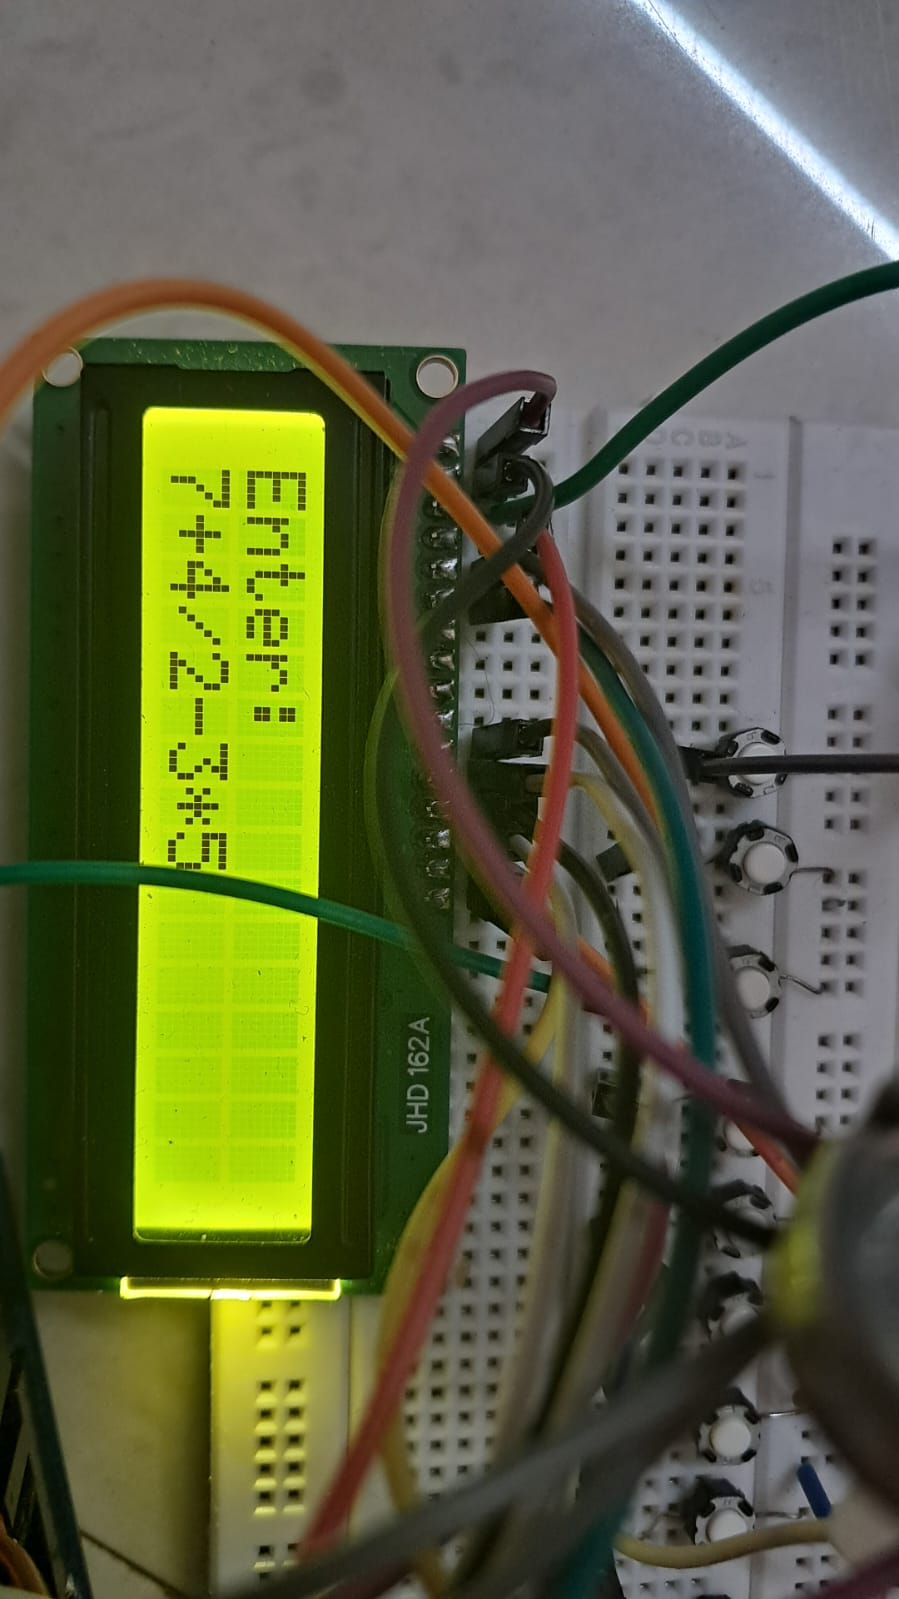
\includegraphics[width = 0.3\textwidth]{figs/exp-1.jpeg}}
	\caption{Expression-1}
\end{figure}
\begin{figure}[h!]
	\centering
	\rotatebox[origin=c]{90}{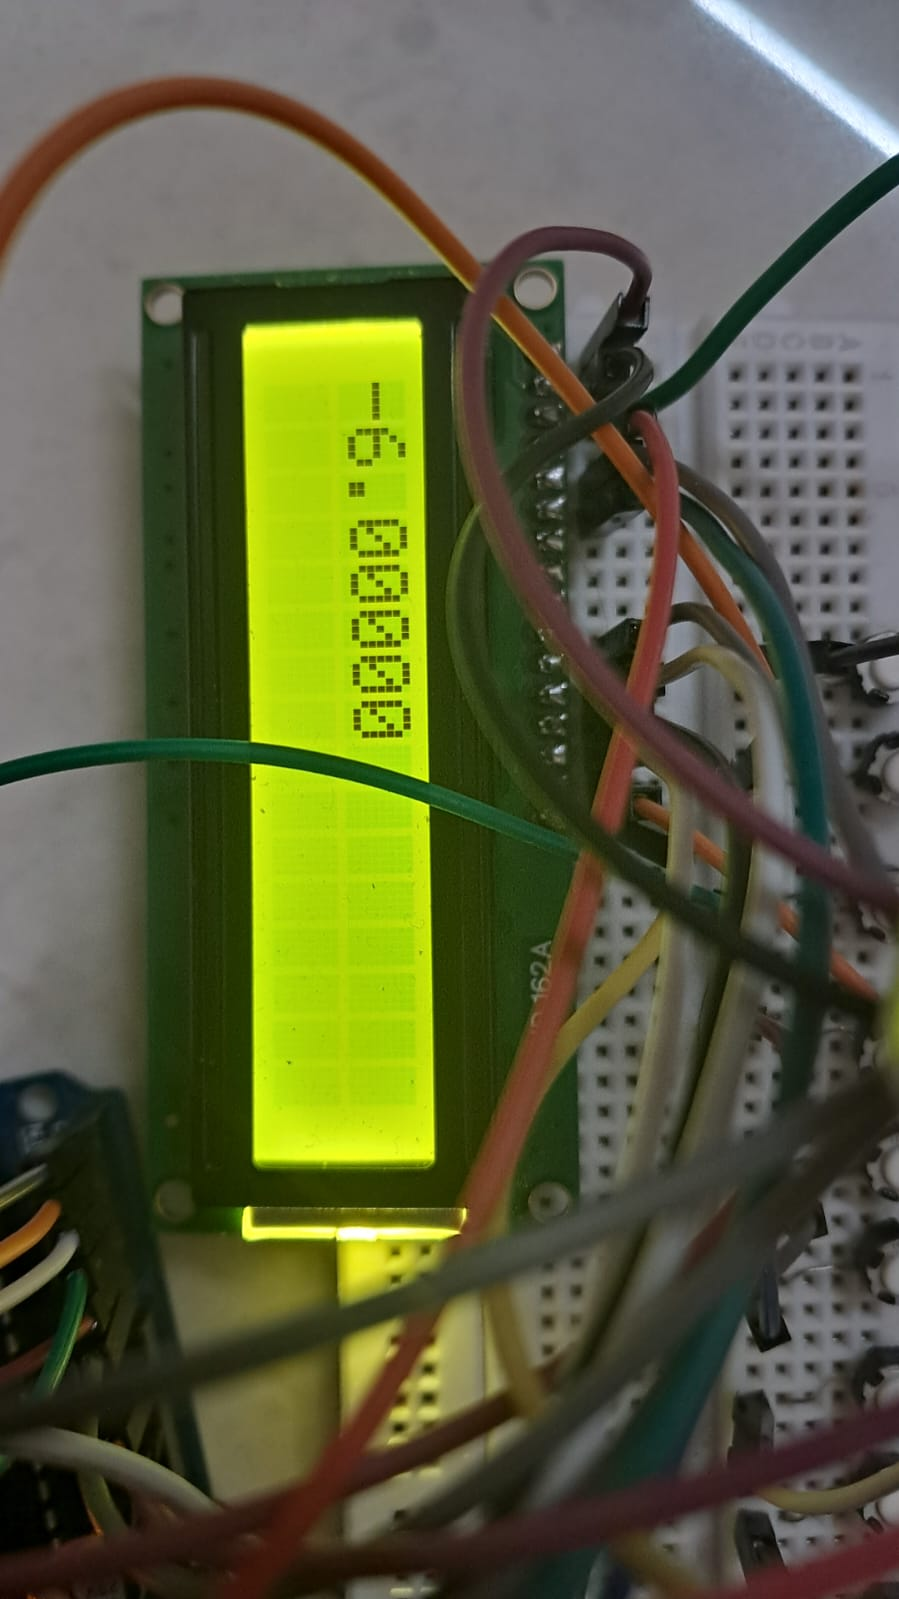
\includegraphics[width = 0.3\textwidth]{figs/res-1.jpeg}}
	\caption{Result-1}
\end{figure}
\begin{figure}[h!]
	\centering
	\rotatebox[origin=c]{90}{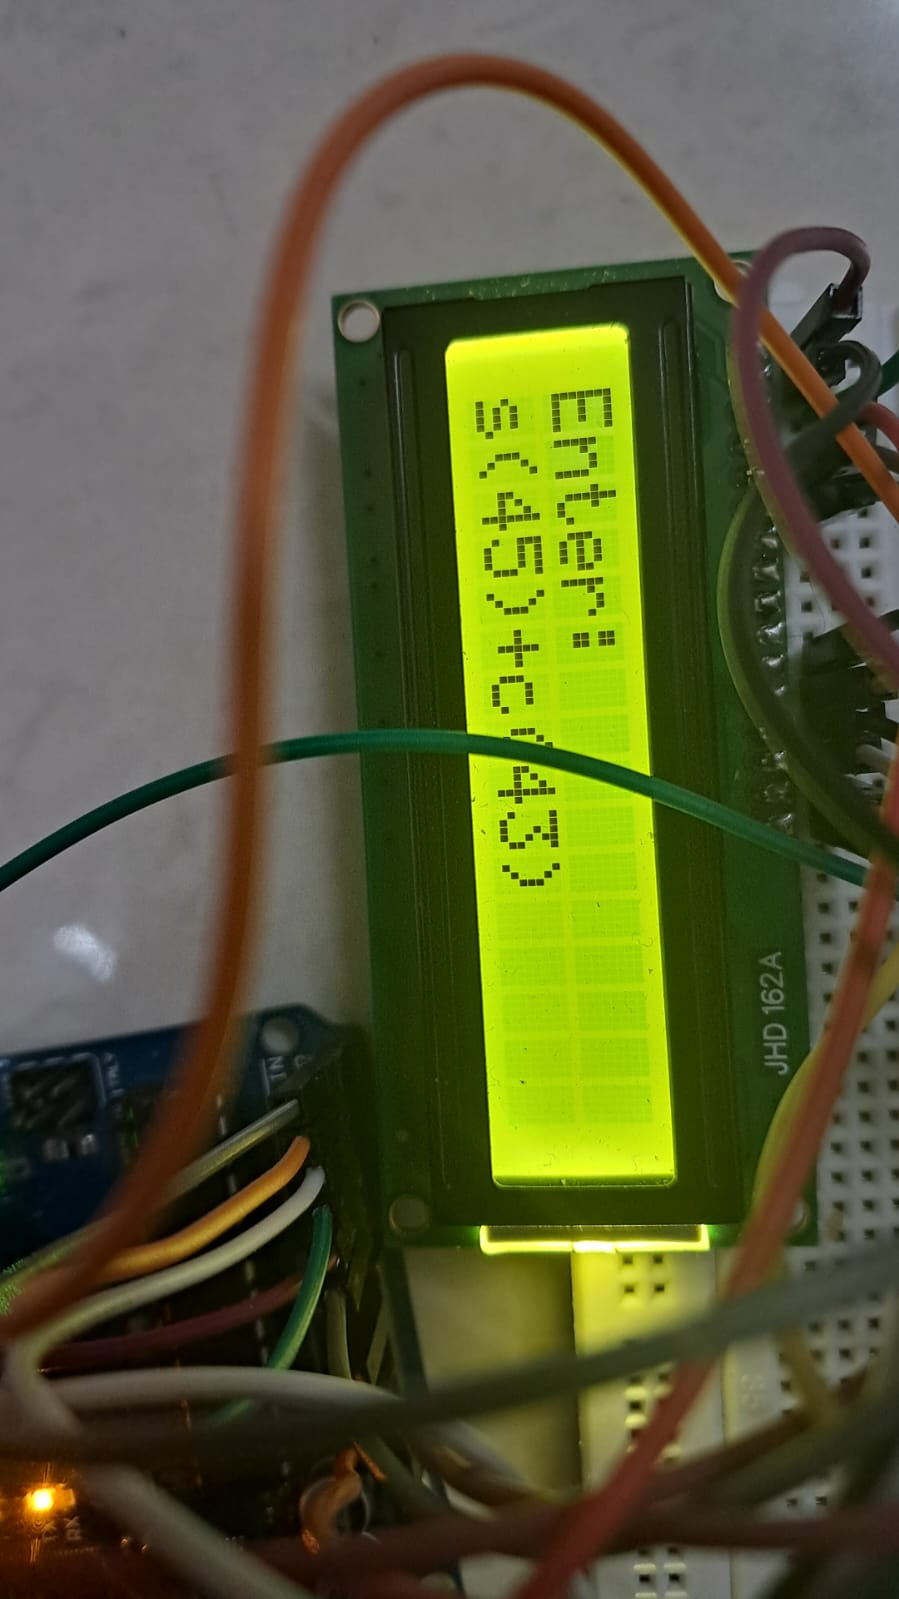
\includegraphics[width = 0.3\textwidth]{figs/exp-2.jpeg}}
	\caption{Expression-2}
\end{figure}
\begin{figure}[h!]
	\centering
	\rotatebox[origin=c]{90}{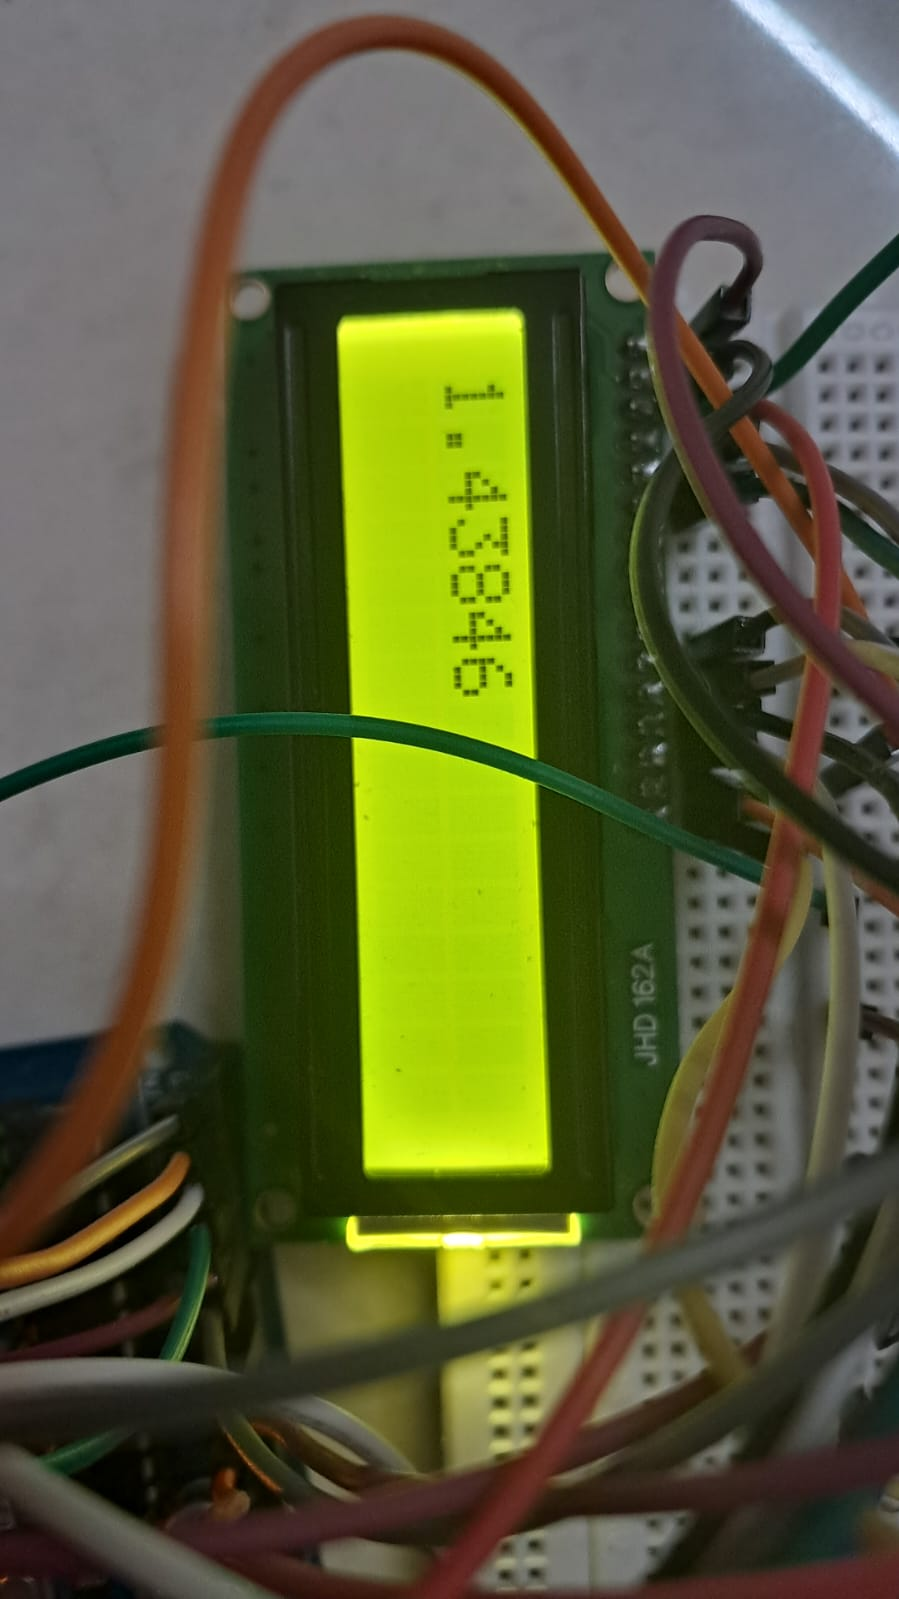
\includegraphics[width = 0.3\textwidth]{figs/res-2.jpeg}}
	\caption{Result-2}
\end{figure}
\pagebreak

\section{Conclusion}
This Arduino-based calculator efficiently evaluates arithmetic and scientific expressions using stacks. The resistor ladder reduces pin usage, and the scrolling feature improves usability. The RK4 method is implemented for trigonometric evaluations, ensuring high accuracy. The calculator ensures efficient parsing, evaluation, and error handling, making it both functional and user-friendly.

\end{document}


